\documentclass{beamer}
\usepackage[utf8]{inputenc}
\usepackage[T1]{fontenc}
\usepackage[ngerman]{babel}
\usepackage{graphicx}
\usepackage{gensymb}
\usepackage{bold-extra}
\usepackage{textcomp}

\input{../flat-blue-theme.inc}

% Make \pause sections invisible
\setbeamercovered{invisible}

\title{OpenStreetMap}
\subtitle{Wat is dat?}
\author{Hauke Stieler\\\href{mailto:4stieler@informatik.uni-hamburg.de}{4stieler@informatik.uni-hamburg.de}}
\titlegraphic{
\includegraphics[width=1.5cm,keepaspectratio]{images/Openstreetmap-logo}}
\date{07. Oktober 2021}

\begin{document}
	\maketitle
	
	\begin{frame}
		\begin{itemize}
			\item So ähnlich wie Google Maps\pause
			\item Aaaaaber: Detailierter, Frei und hat ne Community\pause
			\item Wie Wikipedia nur für Karten\pause
			\item Tausende tolle Apps
		\end{itemize}
	\end{frame}

	\begin{frame}
		\begin{center}
			
\includegraphics[width=0.5\linewidth]{images/happy-meme}
		\end{center}
	\end{frame}
	
	\begin{frame}
		\begin{center}
			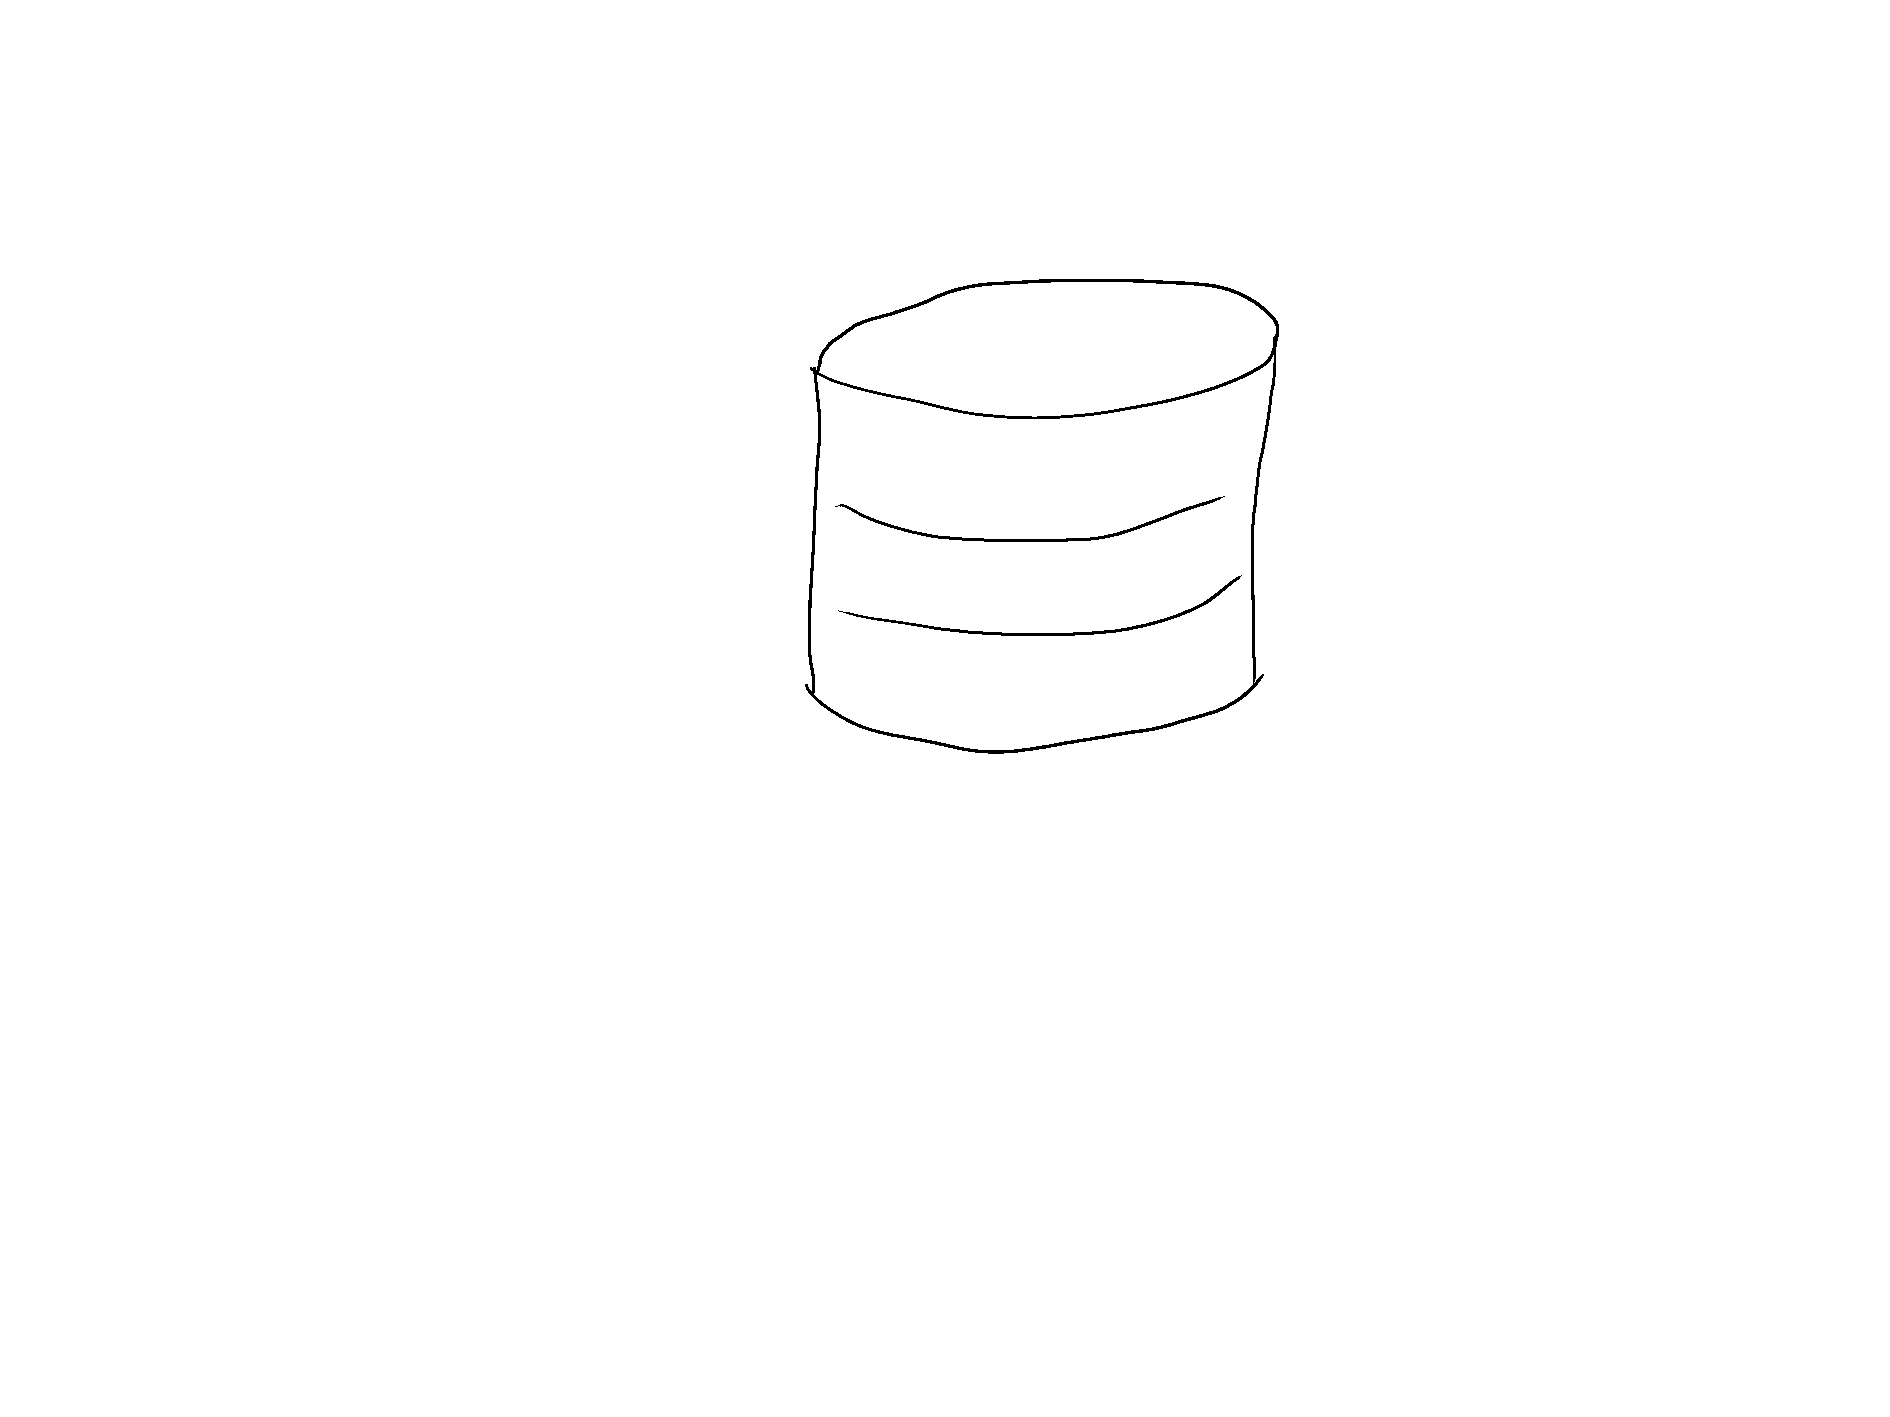
\includegraphics[width=\linewidth]{images/database-1}
		\end{center}
	\end{frame}

	\begin{frame}
		\begin{center}
			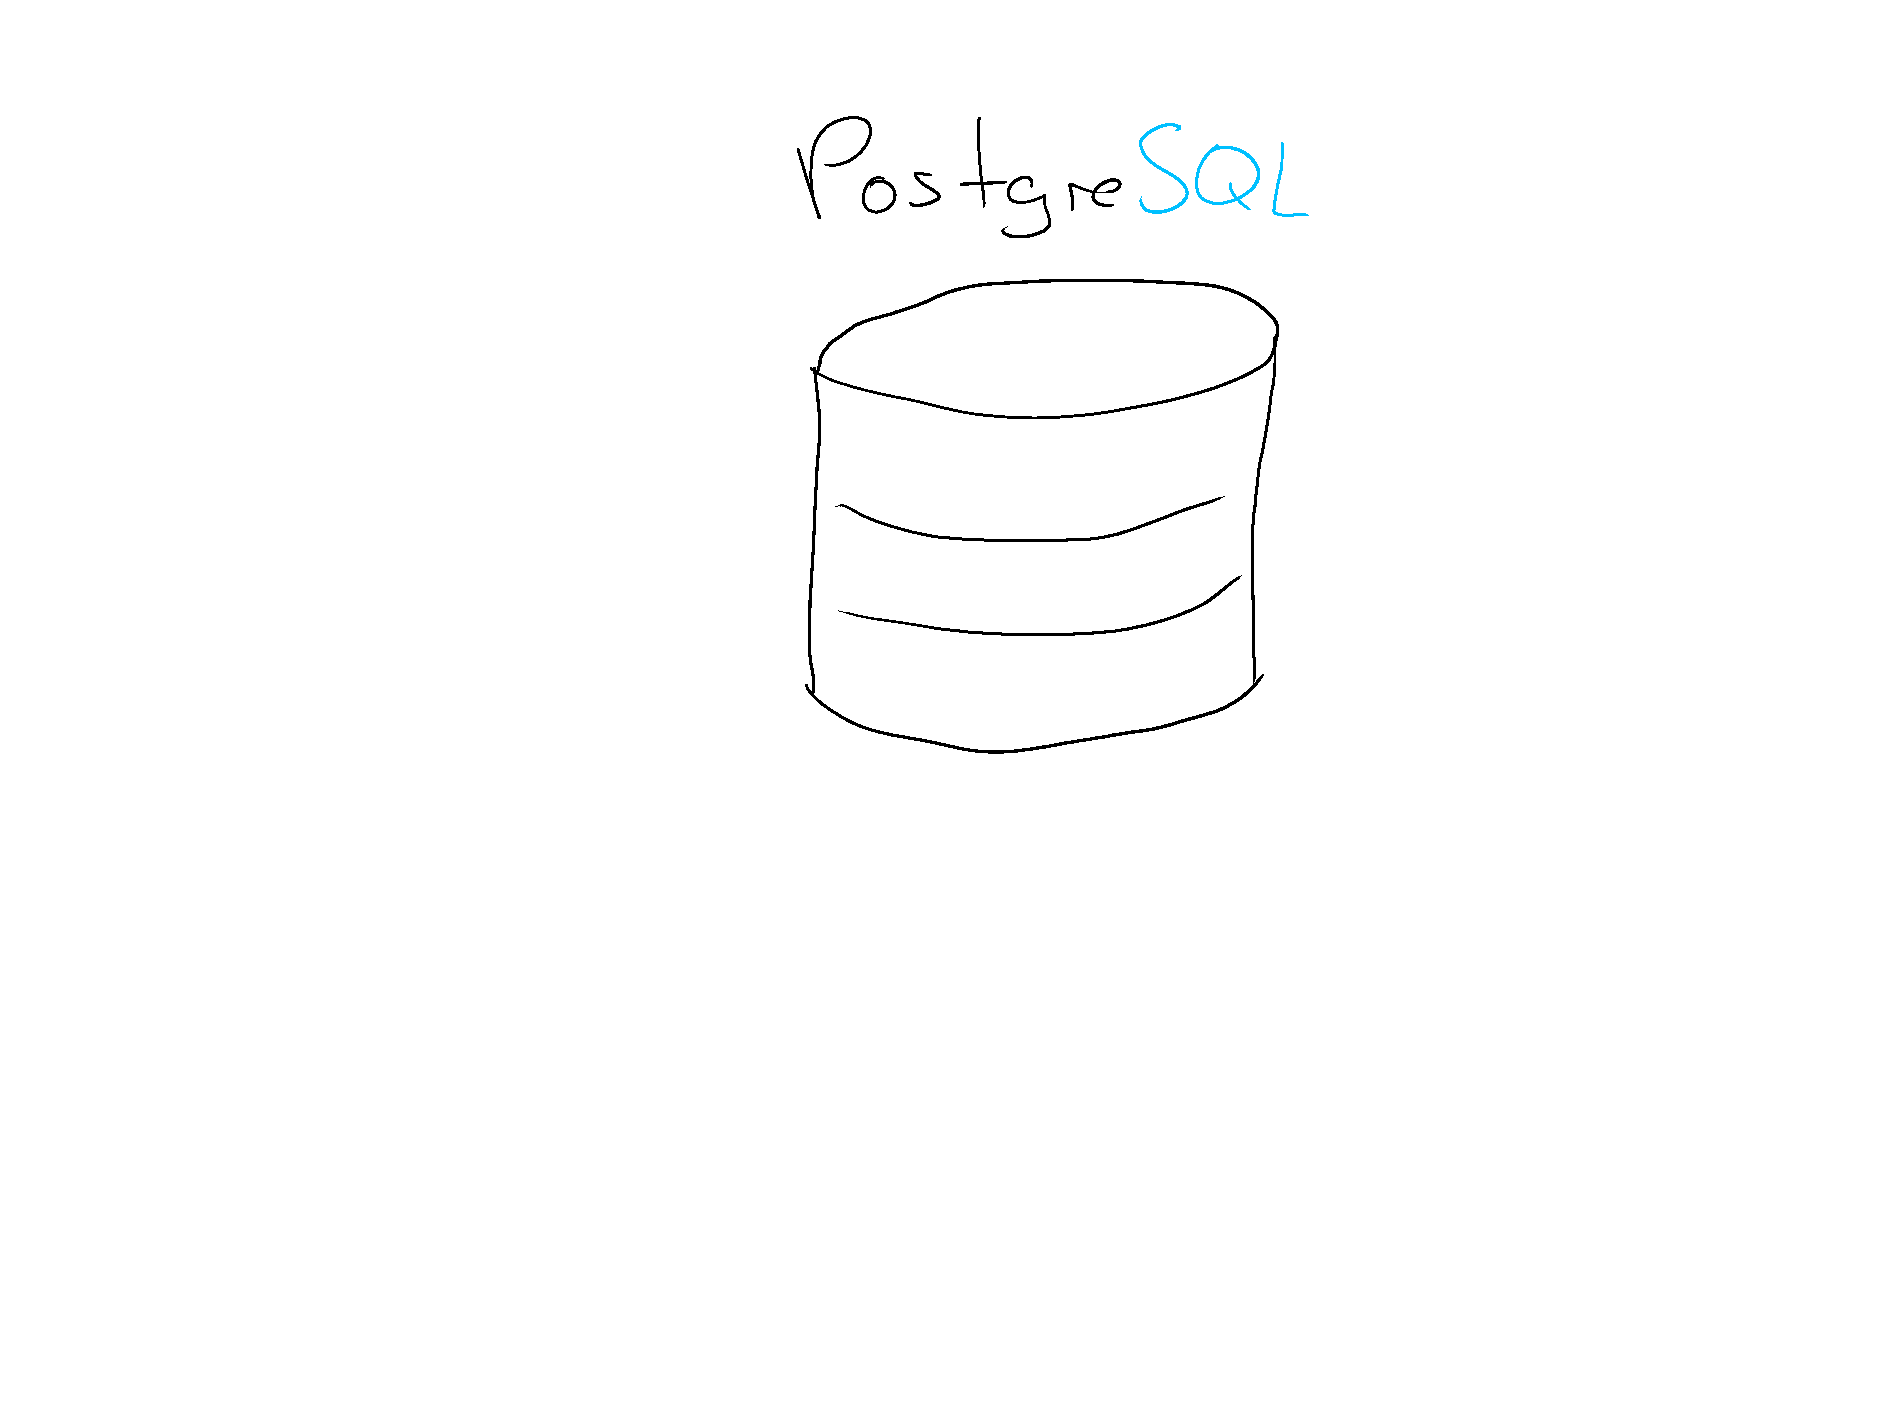
\includegraphics[width=\linewidth]{images/database-2}
		\end{center}
	\end{frame}

	\begin{frame}
		\begin{center}
			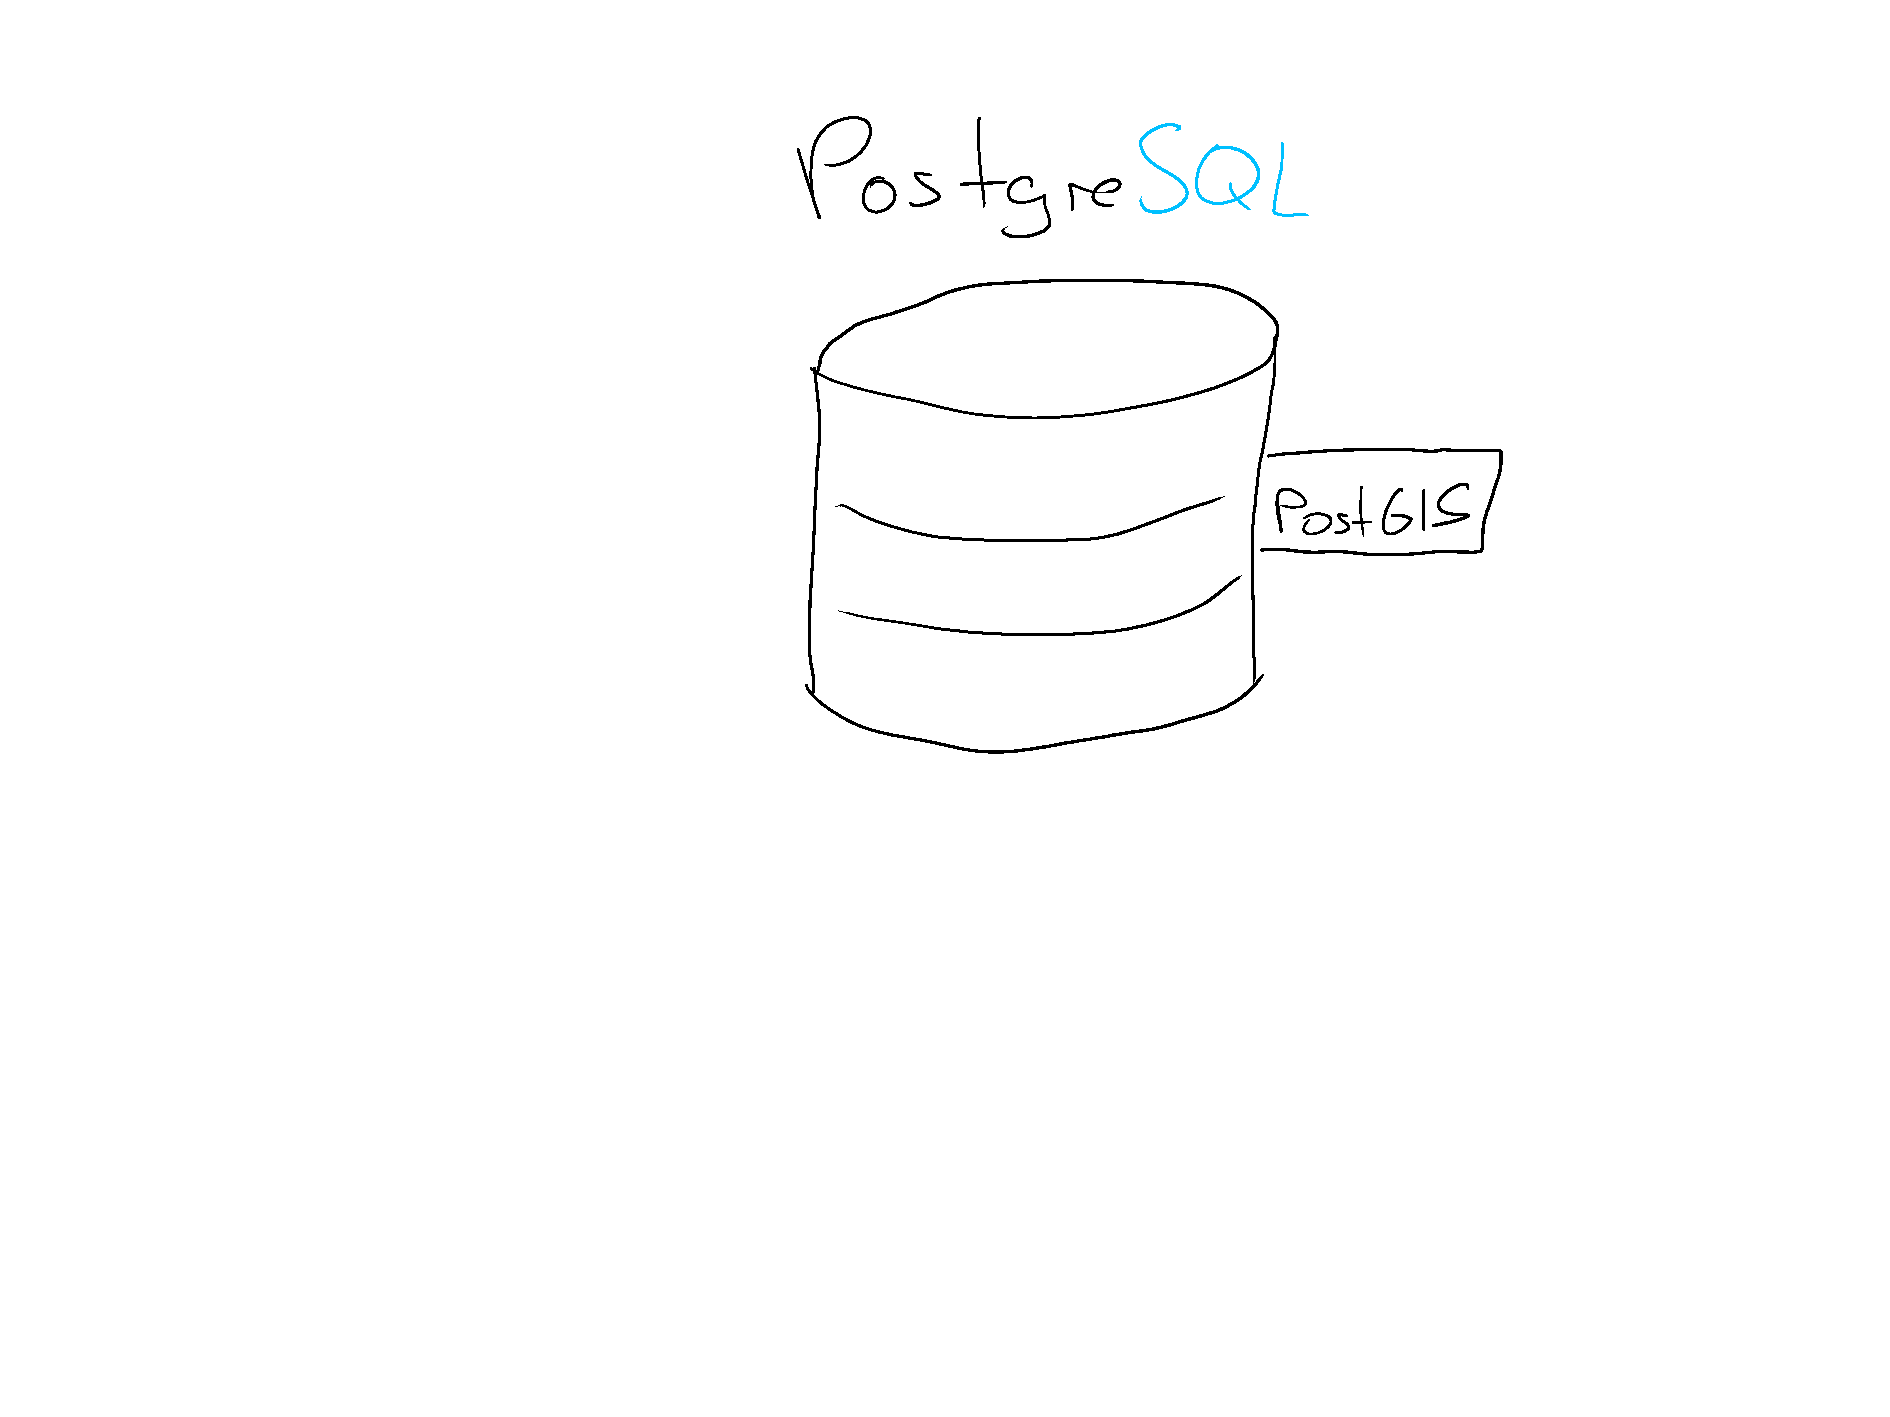
\includegraphics[width=\linewidth]{images/database-3}
		\end{center}
	\end{frame}

	\begin{frame}
		\begin{center}
			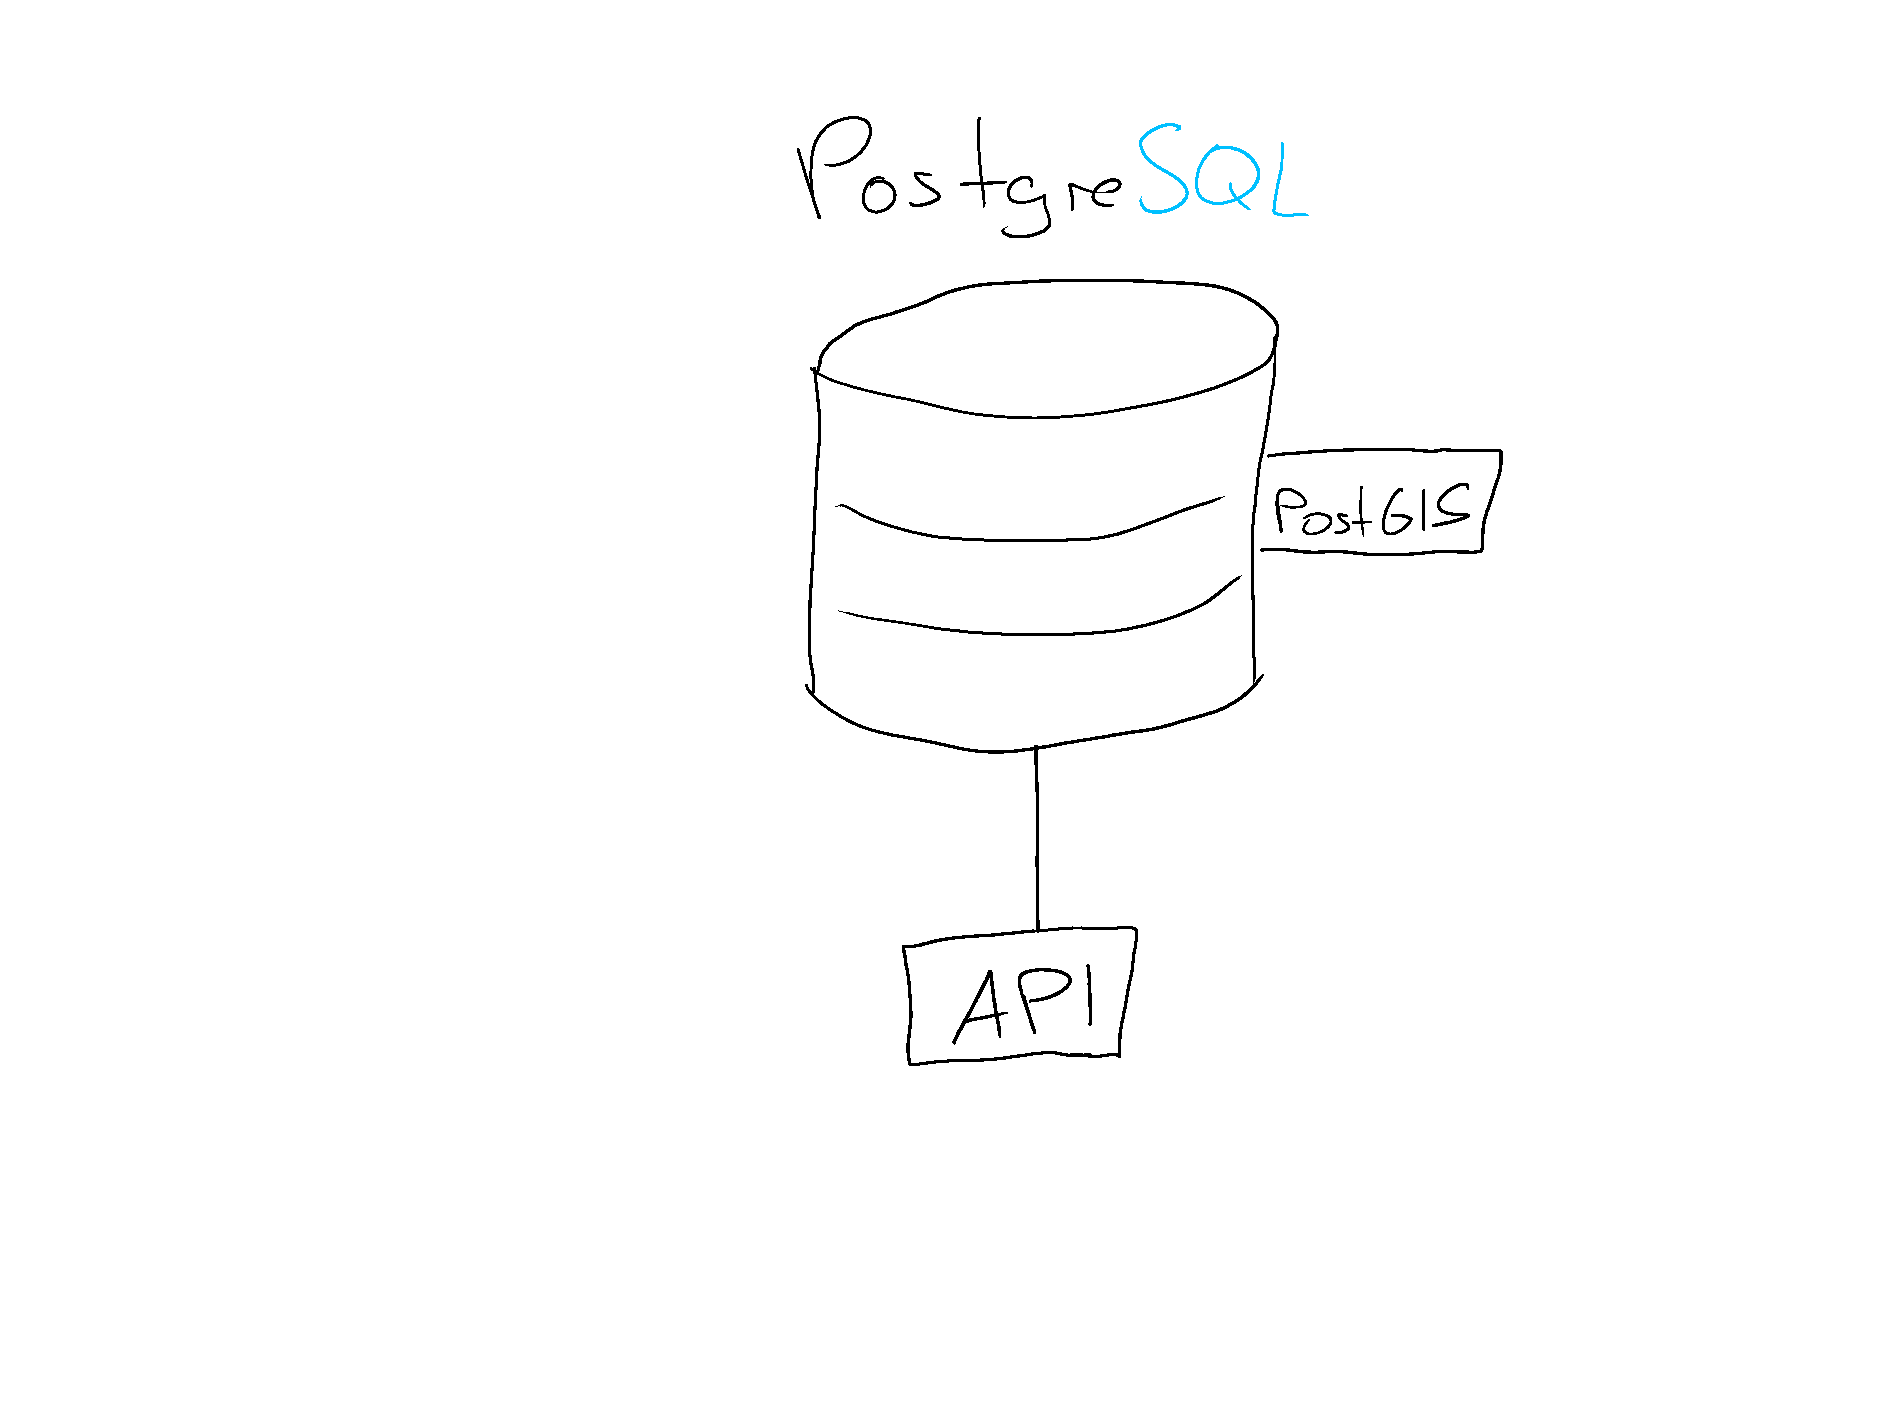
\includegraphics[width=\linewidth]{images/database-4}
		\end{center}
	\end{frame}

	\begin{frame}
		\begin{center}
			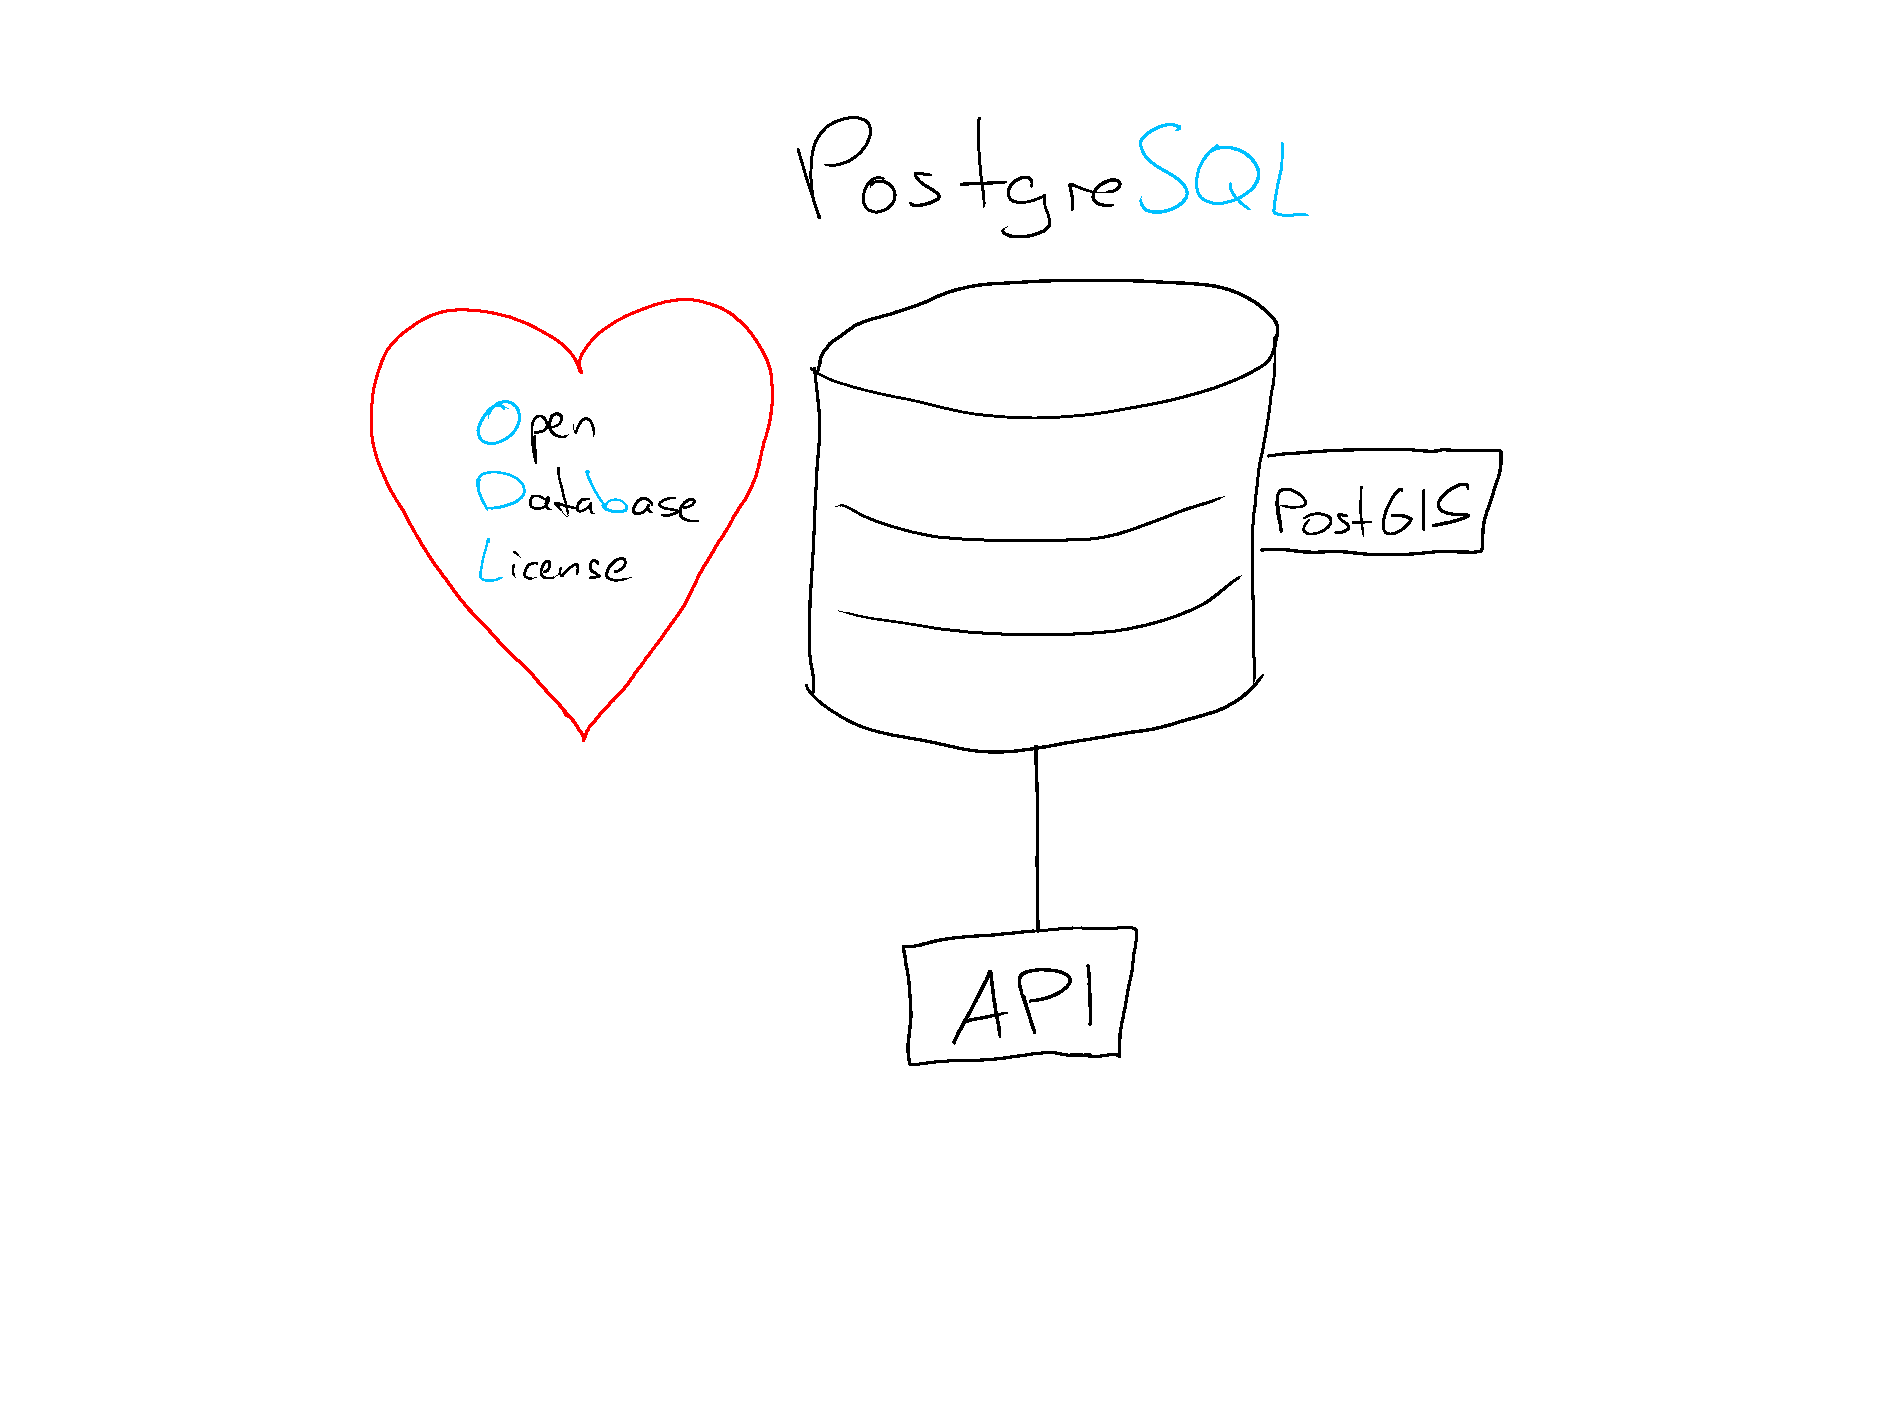
\includegraphics[width=\linewidth]{images/database-5}
		\end{center}
	\end{frame}

	\begin{frame}
		\begin{center}
			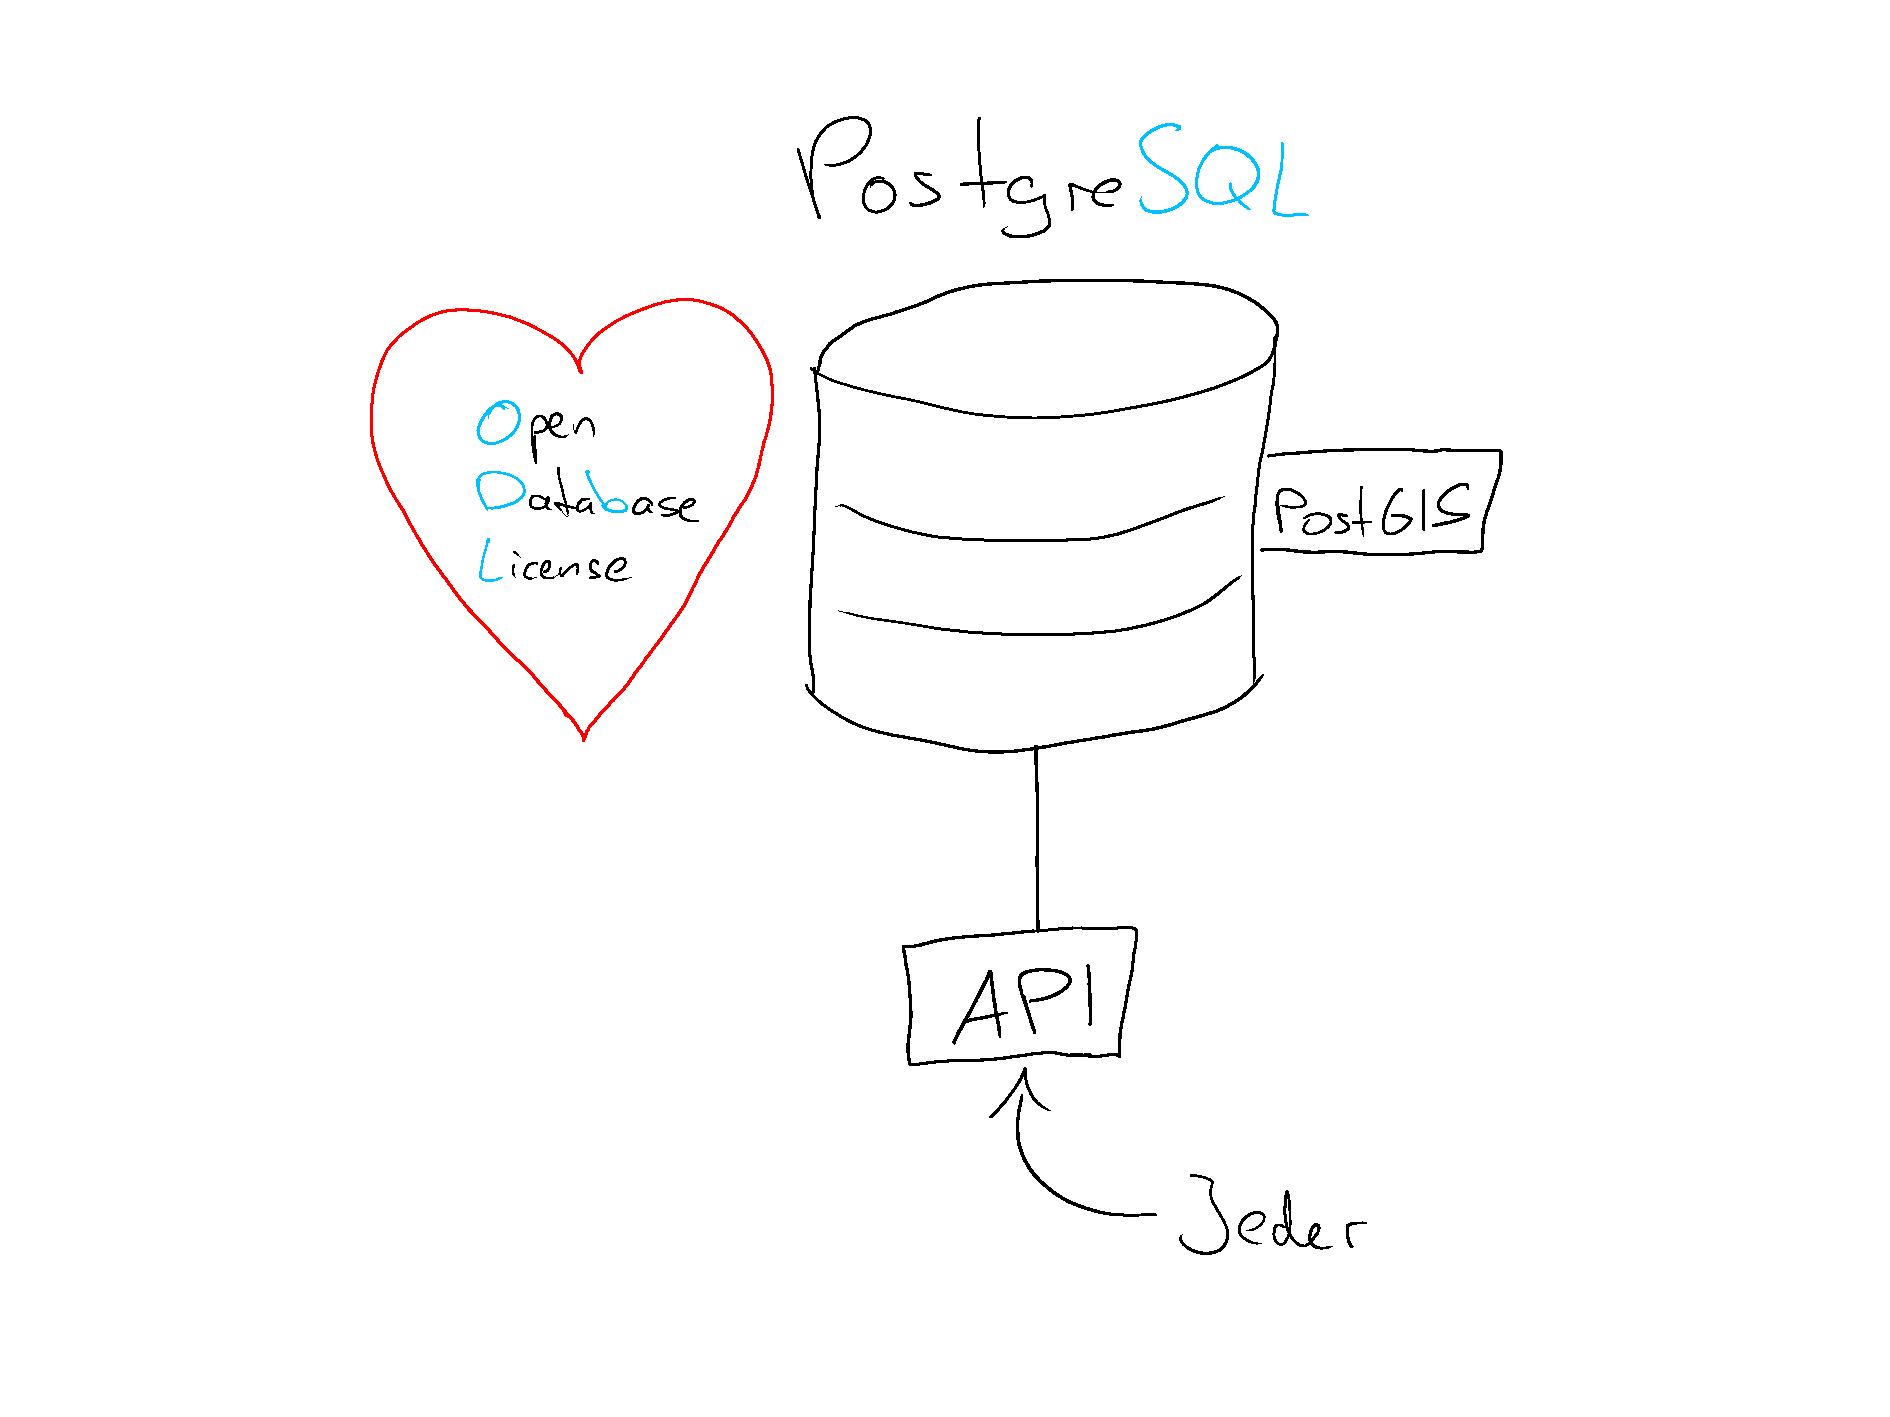
\includegraphics[width=\linewidth]{images/database-6}
		\end{center}
	\end{frame}
	
	
	\begin{frame}
		\begin{center}
			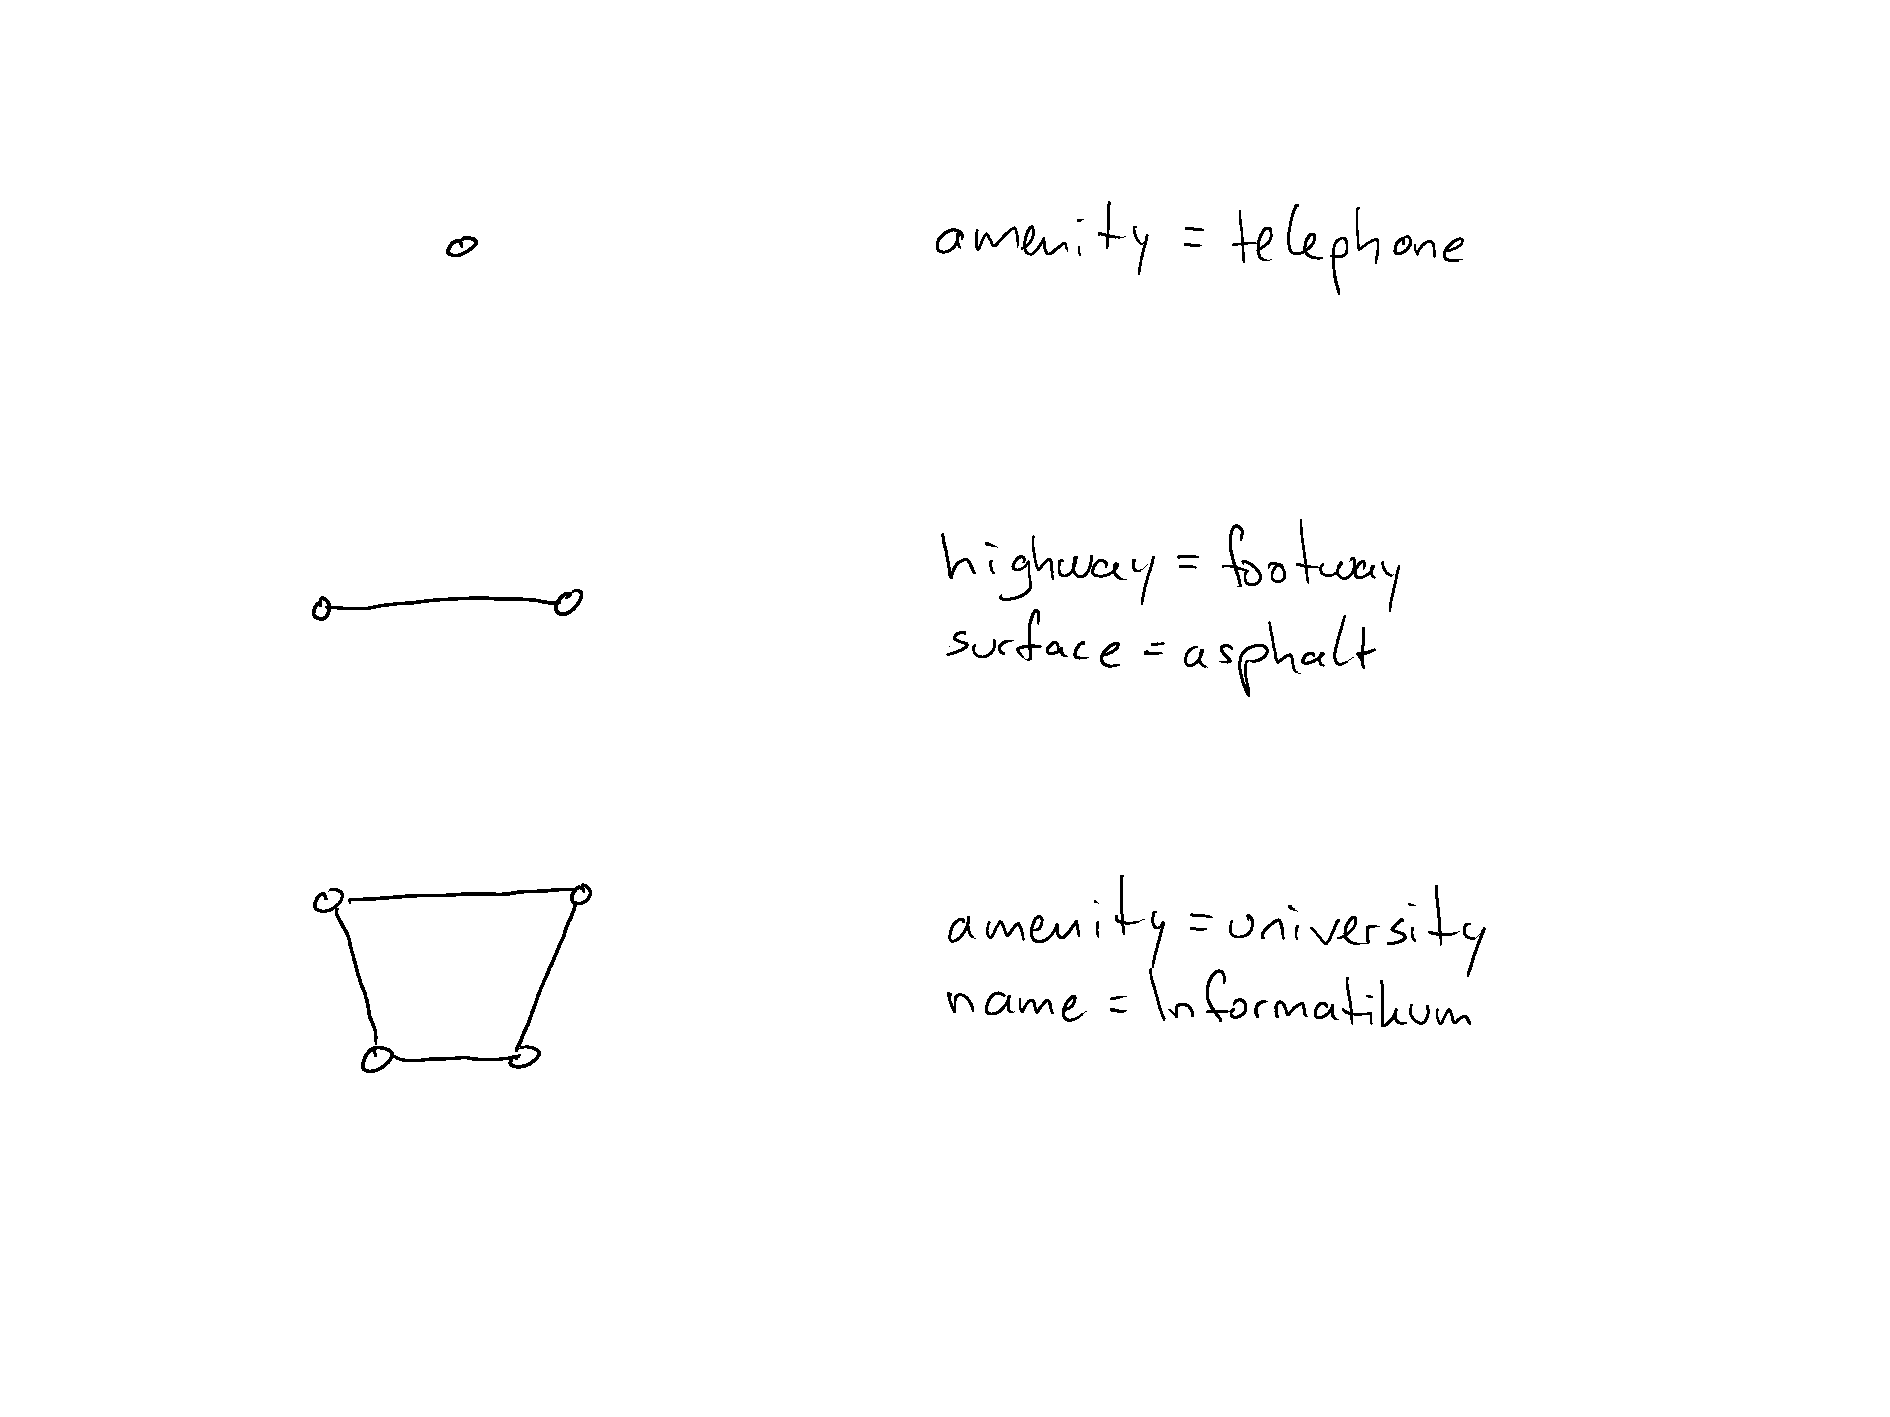
\includegraphics[width=\linewidth]{images/datamodel}
		\end{center}
	\end{frame}
	
	\begin{frame}
		\vspace{1cm}
		\vfill
		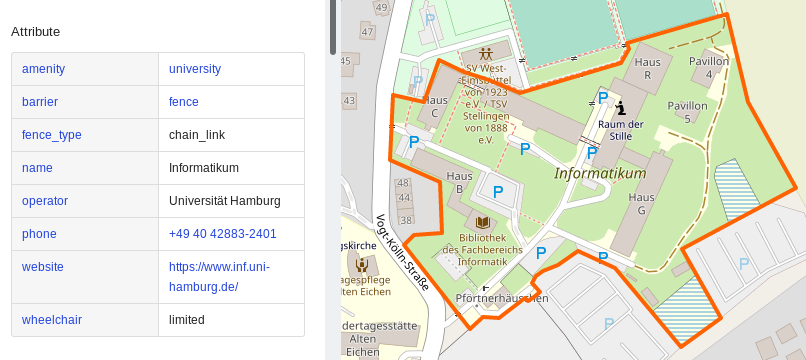
\includegraphics[width=\linewidth]{images/ikum}
		\begin{center}
			{\tiny \copyright{} OpenStreetMap Mitwirkende}
		\end{center}
		\vfill
	\end{frame}

	\begin{frame}
		\vspace{1cm}
		\vfill
		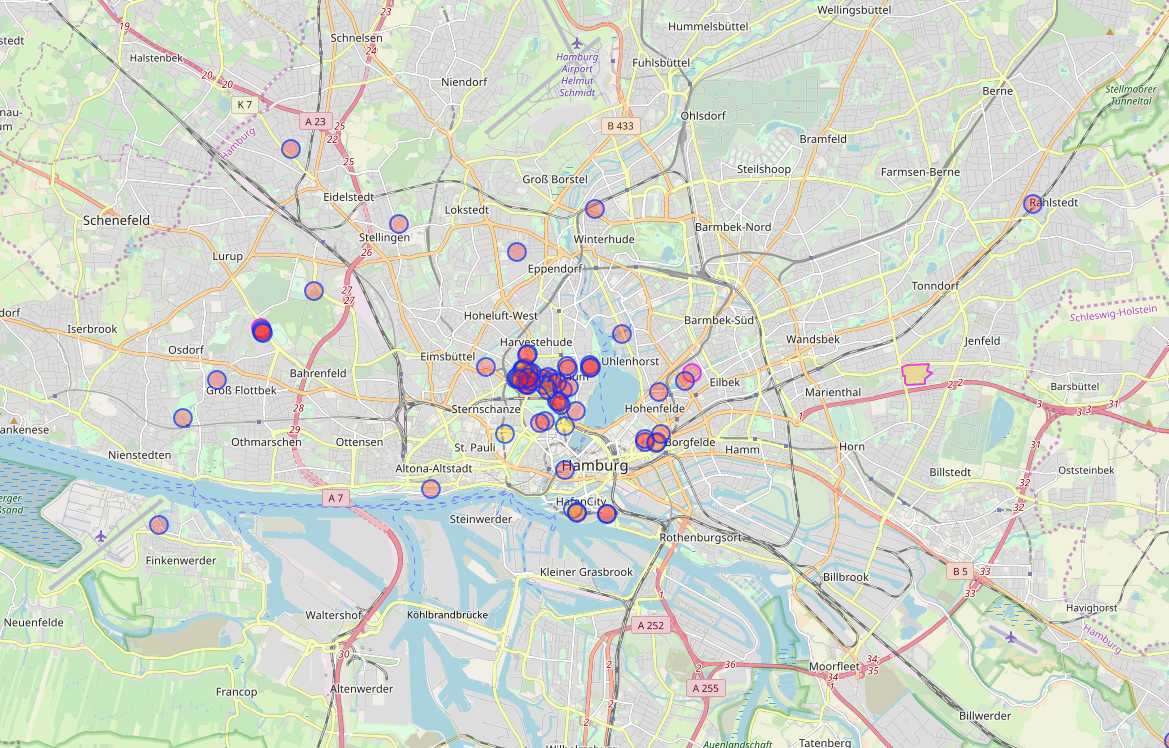
\includegraphics[width=\linewidth]{images/overpass-university}
		\begin{center}
			{\tiny \copyright{} OpenStreetMap Mitwirkende}
		\end{center}
		\vfill
	\end{frame}

	\begin{frame}
		\vfill
		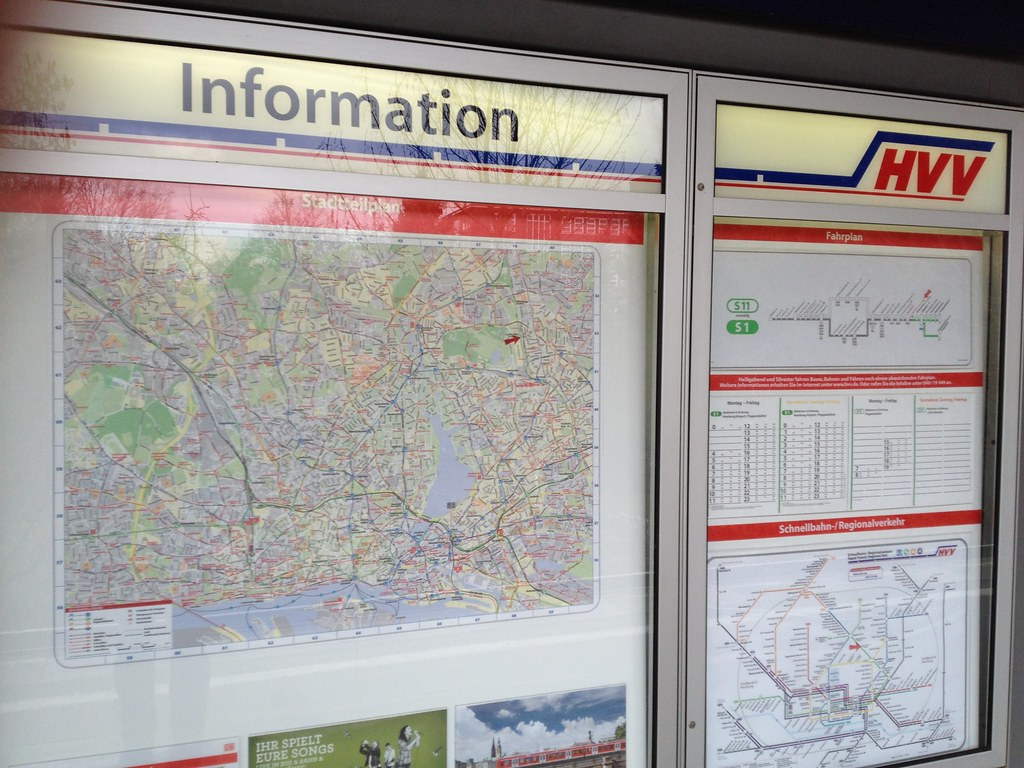
\includegraphics[width=\linewidth]{images/hvv-haltestelle}
		\vfill
	\end{frame}
	
	\begin{frame}
		\vspace{1cm}
		\vfill
		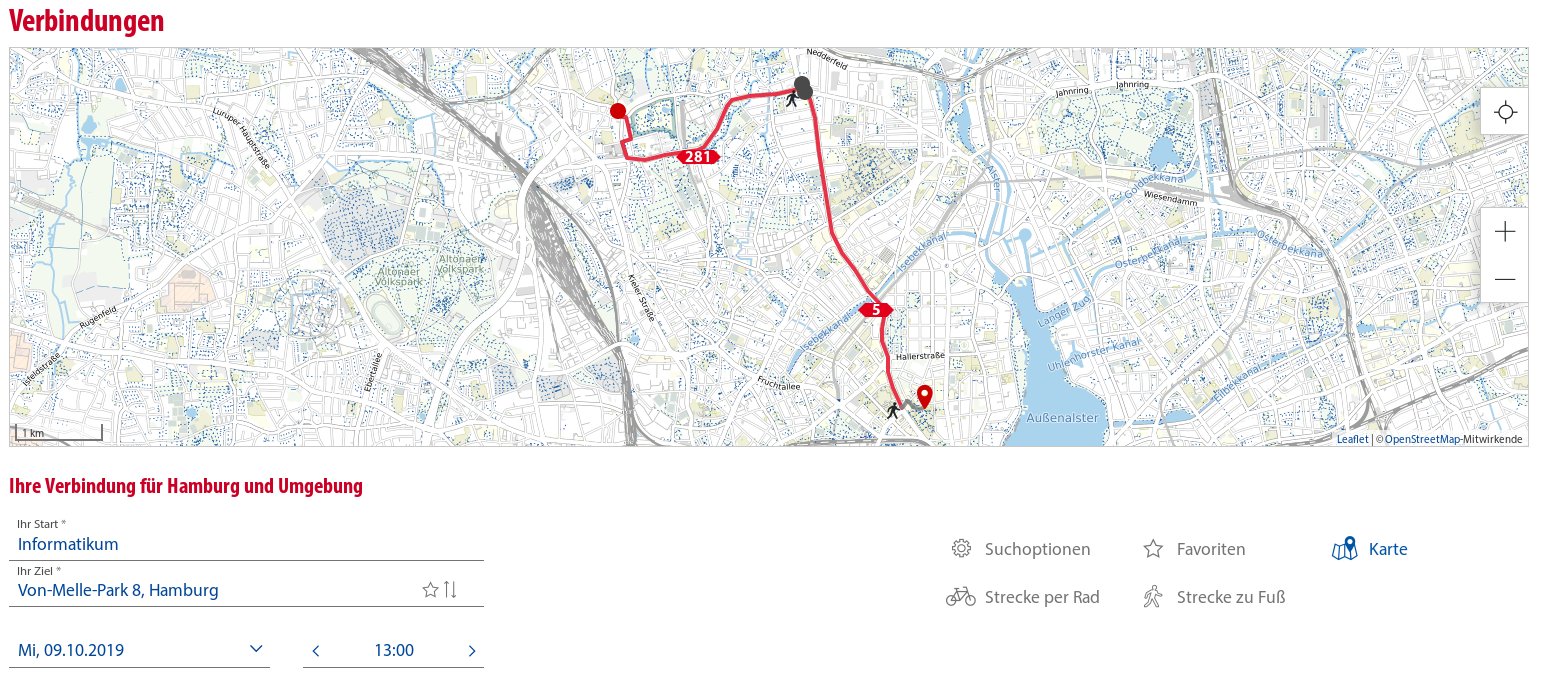
\includegraphics[width=\linewidth]{images/hvv-website}
		\vfill
	\end{frame}

	\begin{frame}
		\vspace{1cm}
		\vfill
		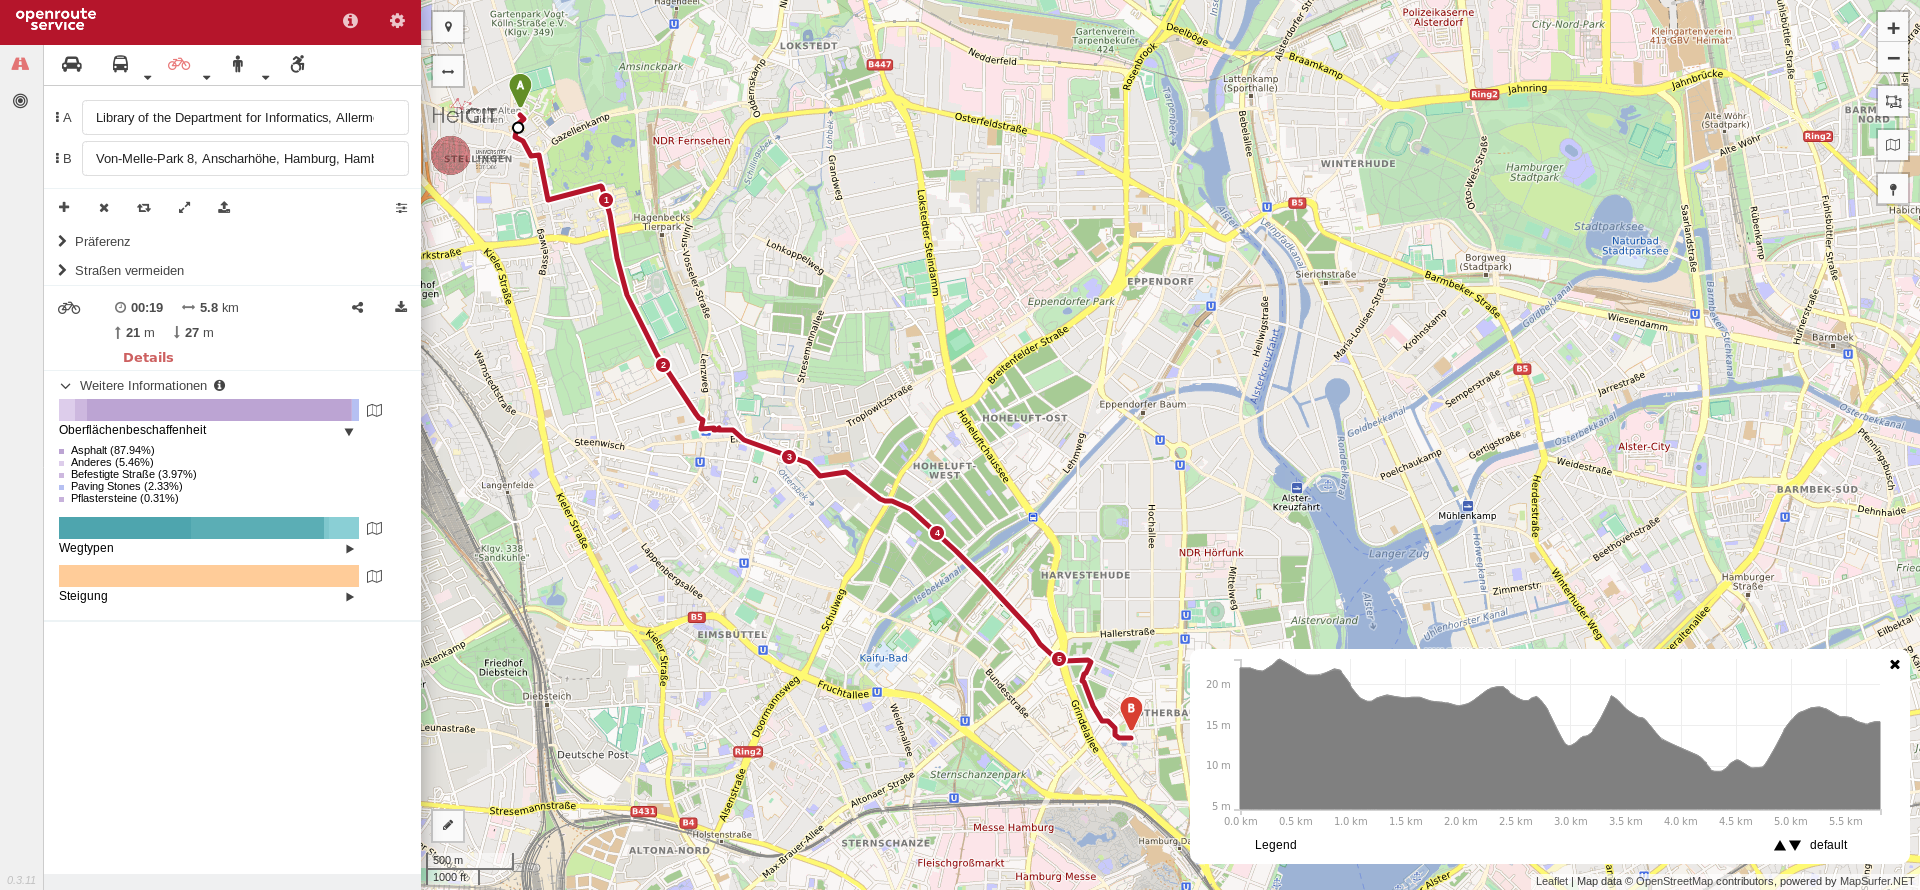
\includegraphics[width=\linewidth]{images/openrouteservice}
		\vfill
	\end{frame}

	\begin{frame}
		\vfill
		\begin{center}
			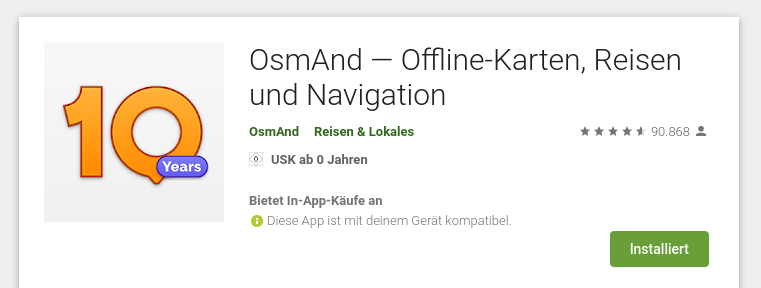
\includegraphics[width=0.7\linewidth]{images/osmand-playstore}\\
			\vspace{0.25cm}
			
\includegraphics[width=0.7\linewidth]{images/organic-maps-playstore}\\
			\vspace{0.25cm}
			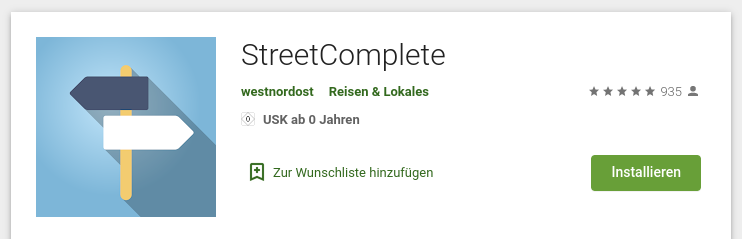
\includegraphics[width=0.7\linewidth]{images/osm-sc-playstore}
		\end{center}
		\vfill
	\end{frame}

	\begin{frame}
		\begin{center}
			
\includegraphics[width=0.5\linewidth]{images/happy-meme-2}
		\end{center}
	\end{frame}

	\begin{frame}
		\vfill
		\begin{center}
			
\includegraphics{images/osm-wiki-org}\\
			\vspace{0.5cm}
			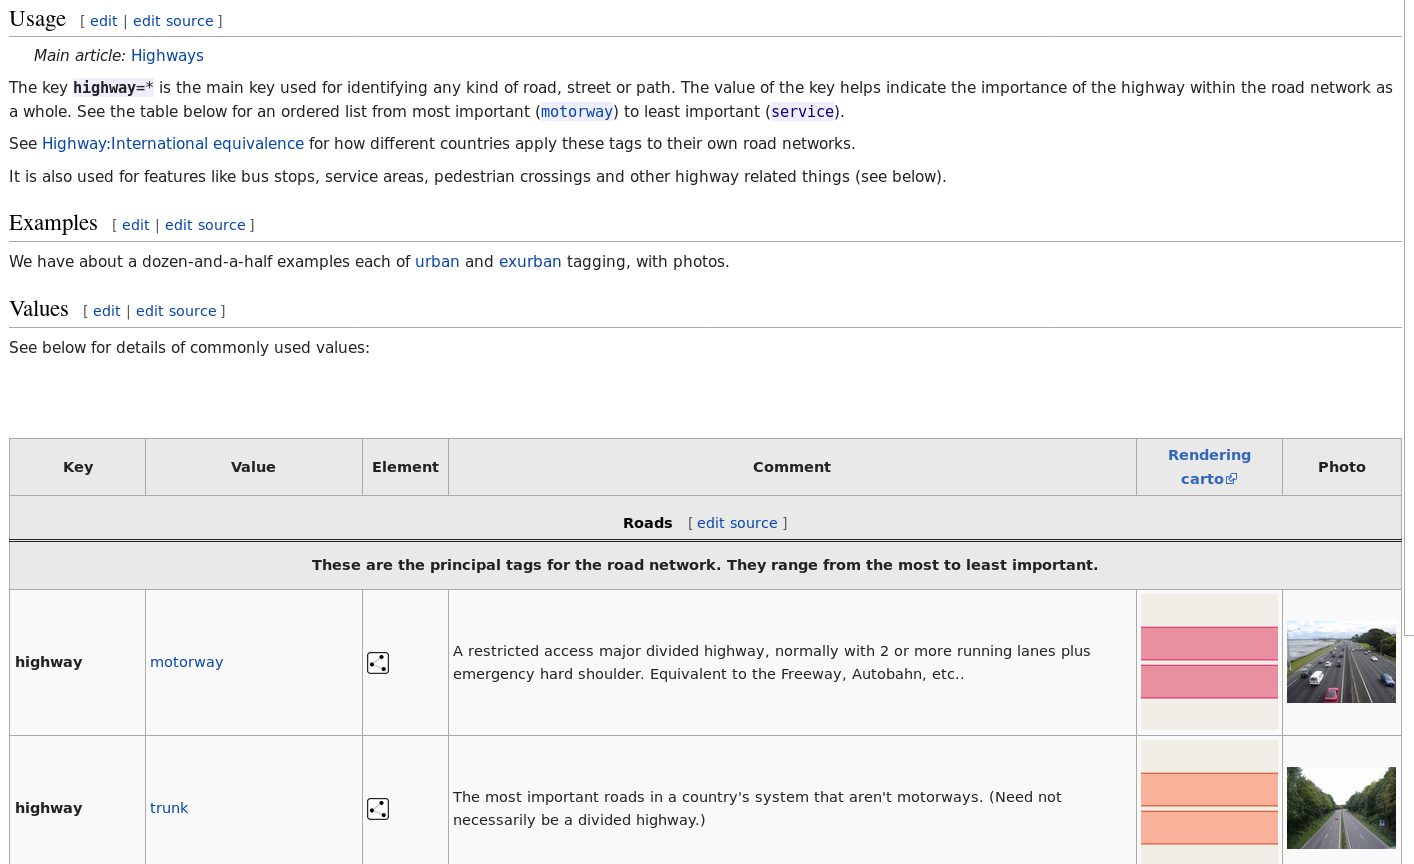
\includegraphics[width=\linewidth]{images/osm-wiki}
		\end{center}
		\vfill
	\end{frame}

	\begin{frame}
		\vfill
		\begin{center}
			
\includegraphics{images/osm-org}
		\end{center}
		\vfill
	\end{frame}

	\begin{frame}
		\vfill
		\begin{center}
			
\includegraphics{images/osm-sign-up}
		\end{center}
		\vfill
	\end{frame}

	\begin{frame}
		\vfill
		\begin{center}
			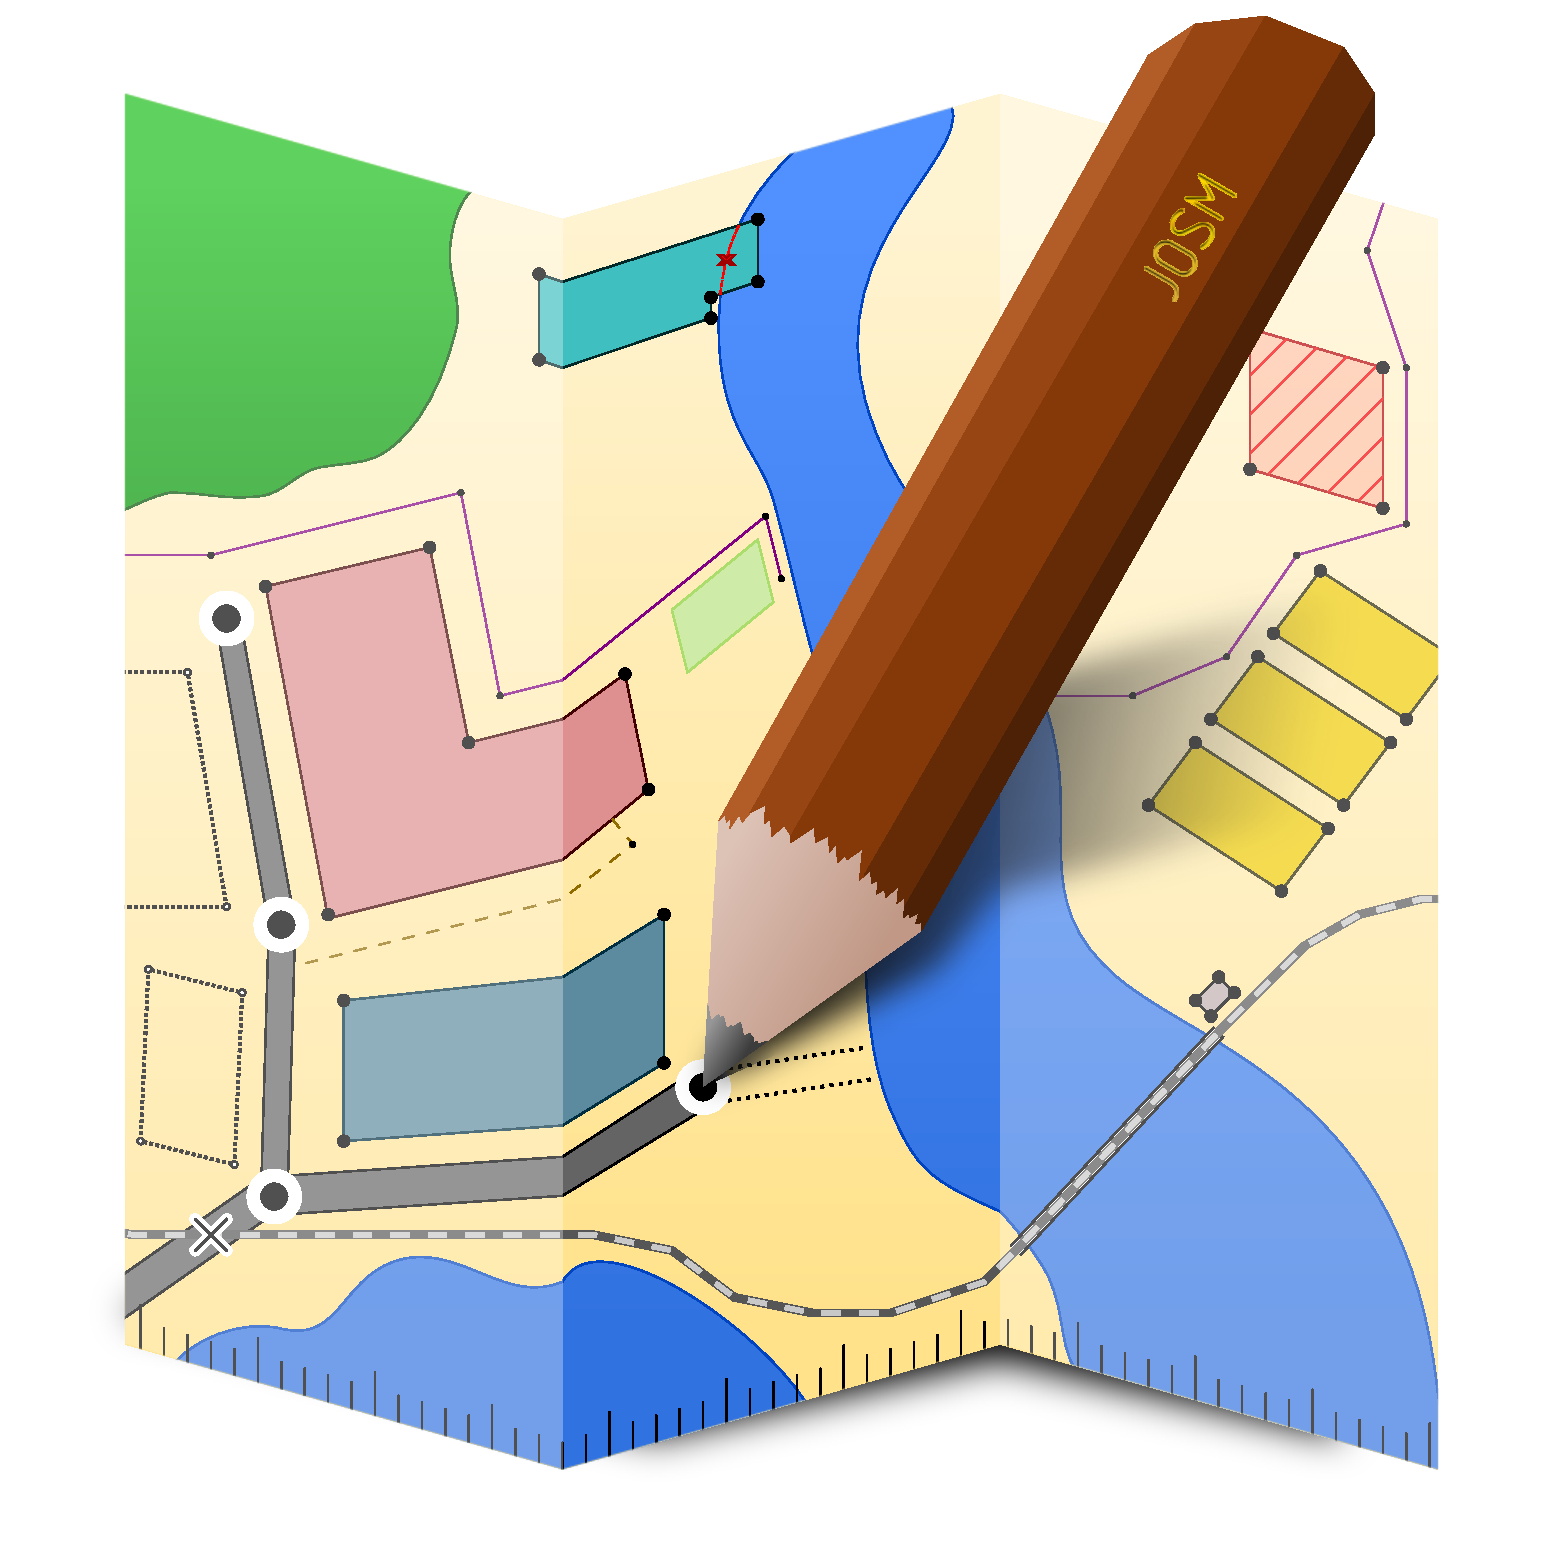
\includegraphics[width=3cm]{images/josm}\\
			JOSM - \textbf{J}ava \textbf{O}pen\textbf{S}treet\textbf{M}ap Editor
		\end{center}
		\vfill
	\end{frame}

	\begin{frame}
		\vfill
		\vspace{0.5cm}
		\hspace*{-1.2cm}
		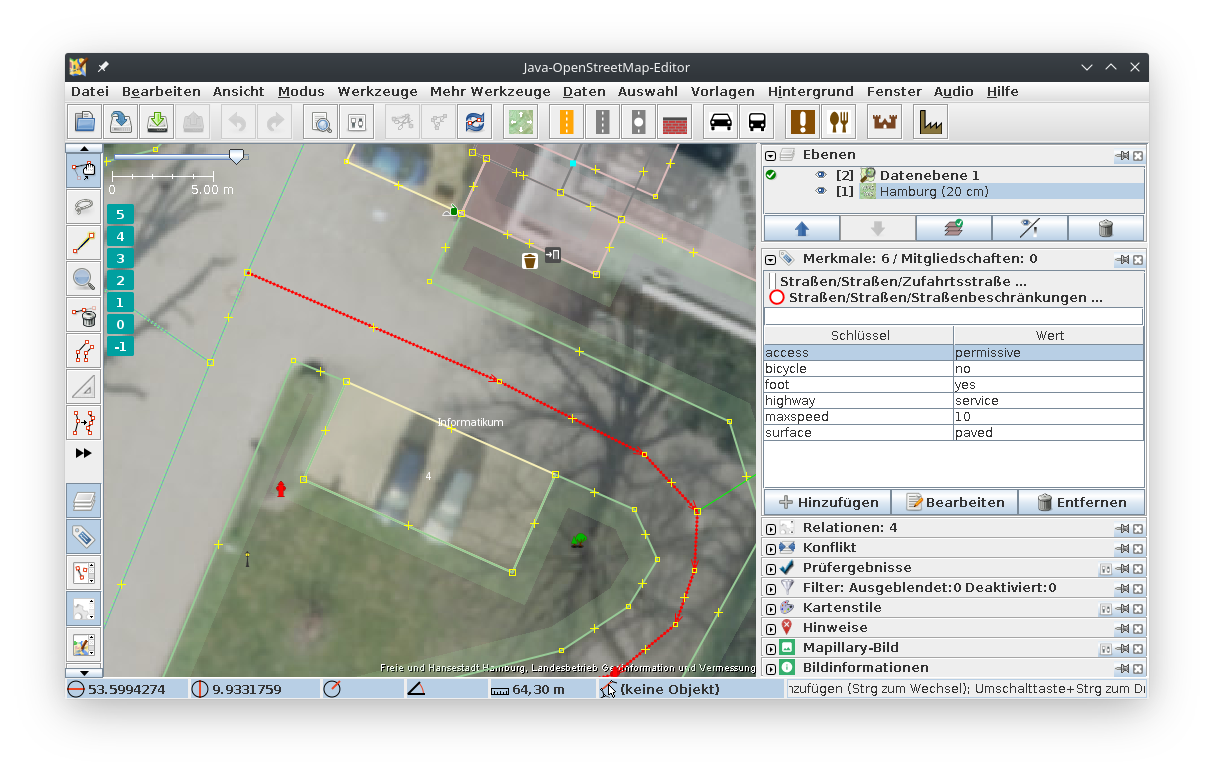
\includegraphics[width=1.2\linewidth]{images/ikum-josm}
		\vfill
	\end{frame}

	\begin{frame}
		\begin{center}
			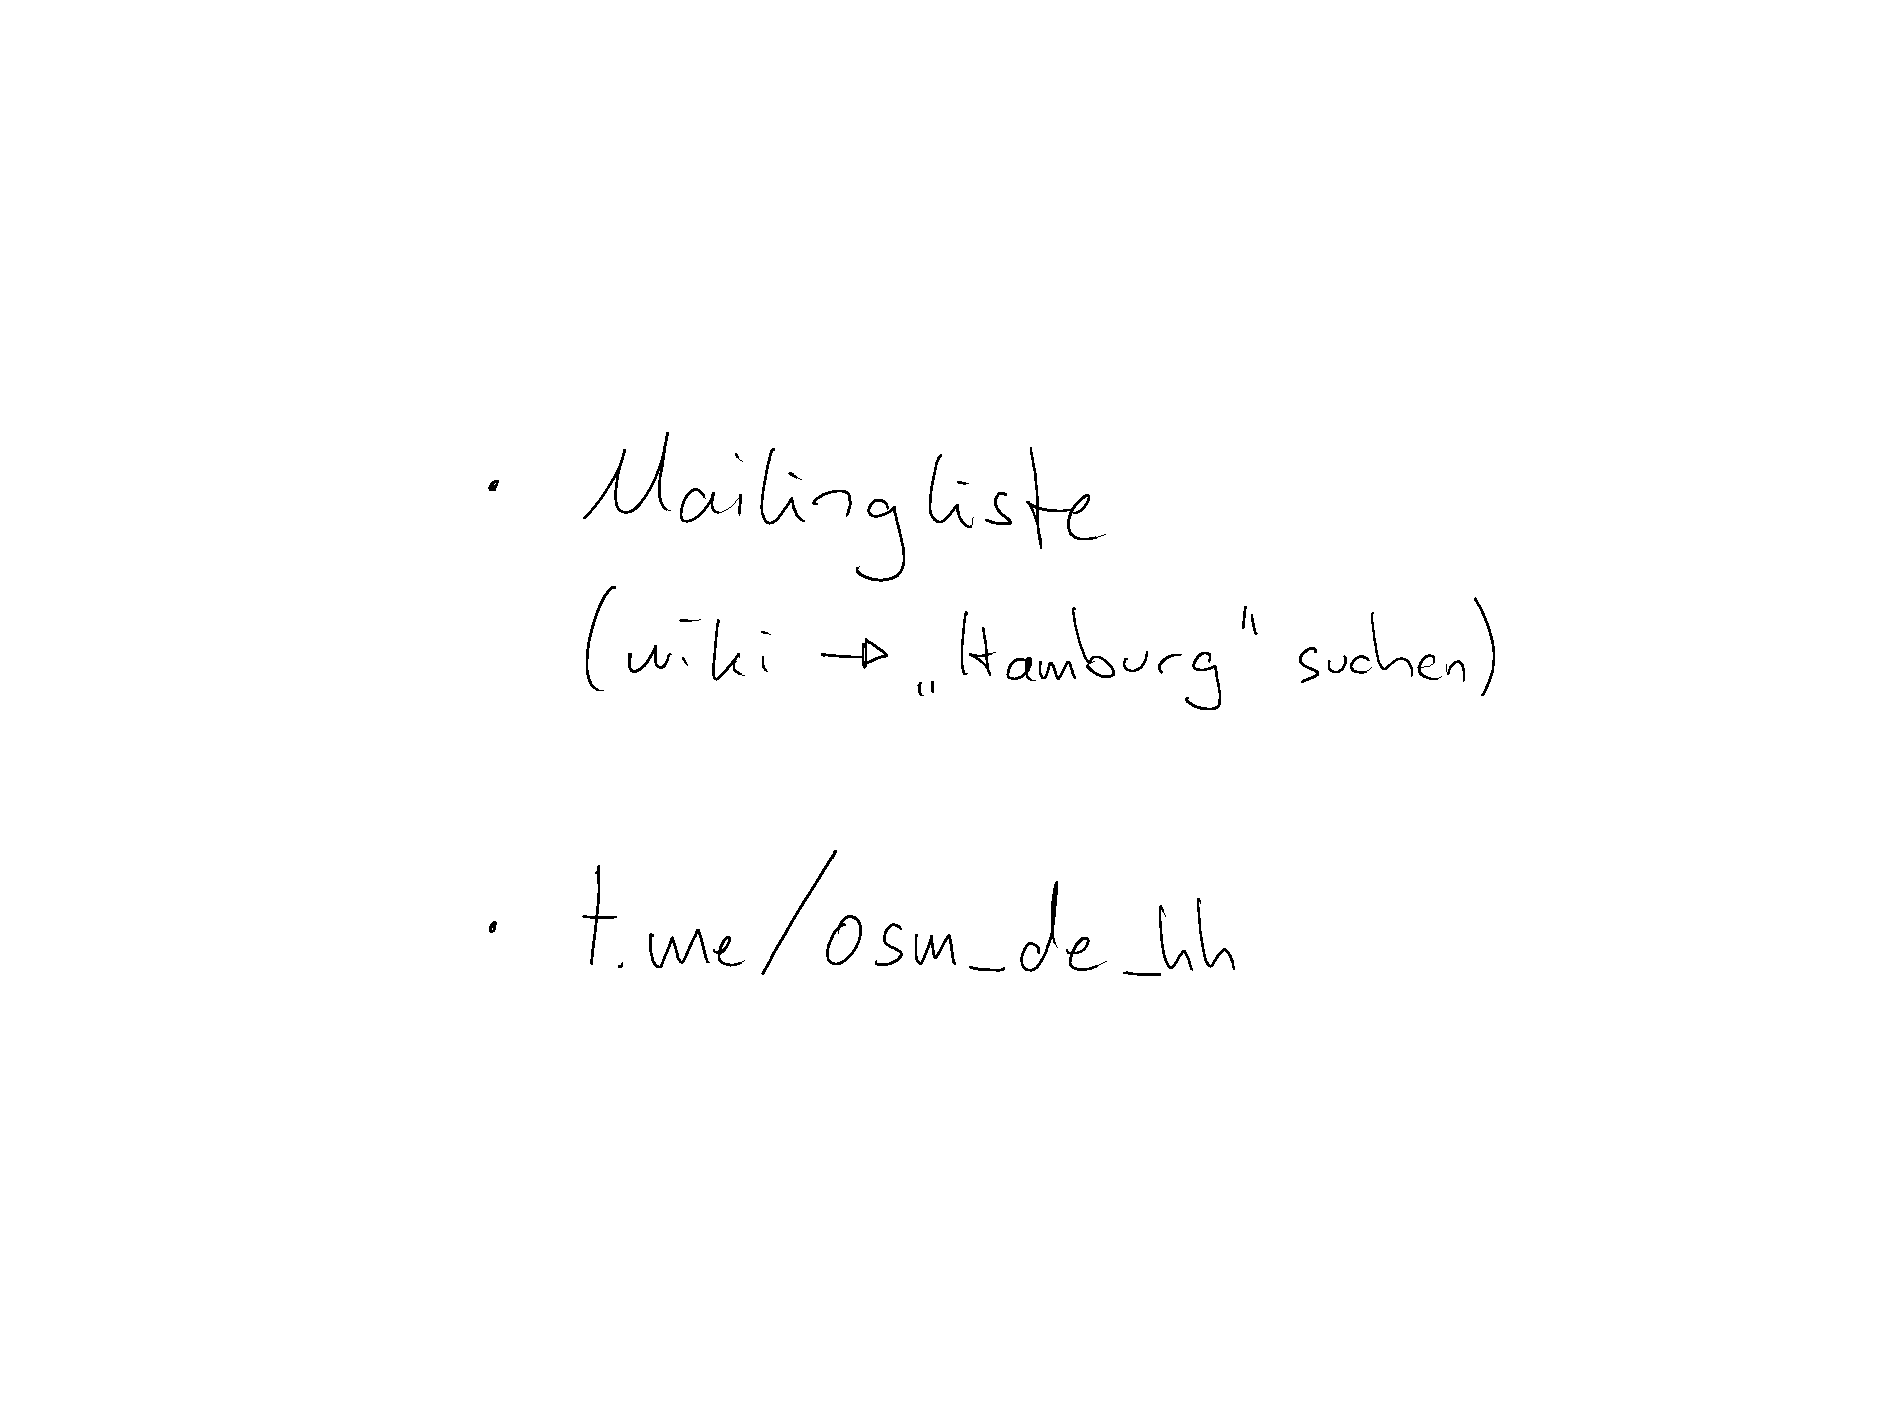
\includegraphics[width=\linewidth]{images/contact}
		\end{center}
	\end{frame}

	\begin{frame}
		\begin{center}
			
\includegraphics[width=\linewidth]{images/danke}
		\end{center}
	\end{frame}
\end{document}